\documentclass{standalone}
\usepackage{tikz}
\usepackage{tikz-qtree}
\usepackage[makeroom]{cancel}
\usetikzlibrary{fit}

% ОПИСАНИЕ: рекурсивный поиск схожести подвыражений
\begin{document} 
	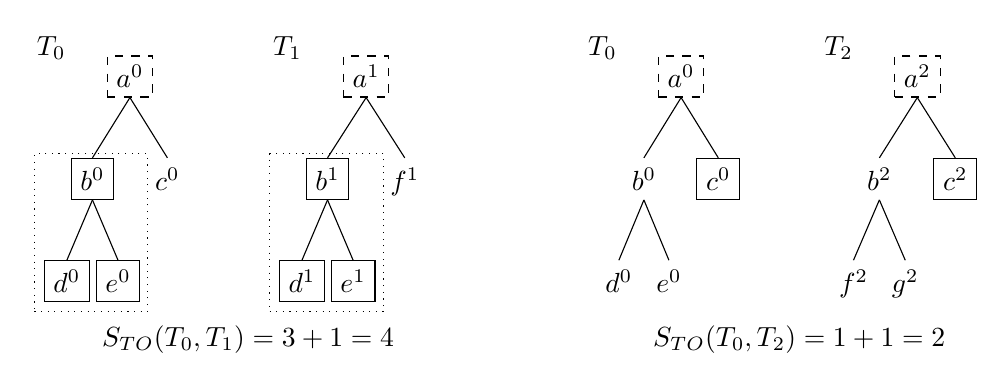
\begin{tikzpicture}[level distance=1.3cm]
		\node (Sto1) at (1.5,-3.2) {$S_{TO}(T_0,T_1) = 3 + 1 = 4$} ;
	    \node (x) at (-1,0.5) {$T_0$} ;
	    \Tree [.\node[draw,dashed]{$a^0$};
	            [.\node[draw]{$b^0$};
	                [.\node(d)[draw]{$d^0$}; ] 
	                [.\node[draw]{$e^0$}; ] 
	            ] 
	            [.$c^0$ ]
	          ]
	    \node (ph) at (-0.15,-1.2) {\phantom{X}};
		\node[draw,dotted,fit=(d)(ph)]{};
	          
	    \begin{scope}[xshift=3cm]
	    \node (y) at (-1,0.5) {$T_1$} ;
	    \Tree [.\node[draw,dashed]{$a^1$};
	            [.\node[draw]{$b^1$};
	                [.\node(d)[draw]{$d^1$}; ] 
	                [.\node[draw]{$e^1$}; ] 
	            ] 
	            [.$f^1$ ]
	          ]
	    \node (ph) at (-0.15,-1.2) {\phantom{X}};
		\node[draw,dotted,fit=(d)(ph)]{};
	    \end{scope}



	    \begin{scope}[xshift=7cm]
	    \node (Sto2) at (1.5,-3.2) {$S_{TO}(T_0,T_2) = 1 + 1 = 2$} ;
	    \node (x) at (-1,0.5) {$T_0$} ;
	    \Tree [.\node[draw,dashed]{$a^0$};
	            [.$b^0$
	                [.$d^0$ ] 
	                [.$e^0$ ] 
	            ] 
	            [.\node[draw]{$c^0$}; ]
	          ]
	    \end{scope}

	    \begin{scope}[xshift=10cm]
	    \node (z) at (-1,0.5) {$T_2$} ;
	    \Tree [.\node[draw,dashed]{$a^2$};
	            [.$b^2$
	                [.$f^2$ ] 
	                [.$g^2$ ] 
	            ] 
	            [.\node[draw]{$c^2$}; ]
	          ]
	    \end{scope}


	\end{tikzpicture}
\end{document} 